\begin{center}
\begin{figure}[H]
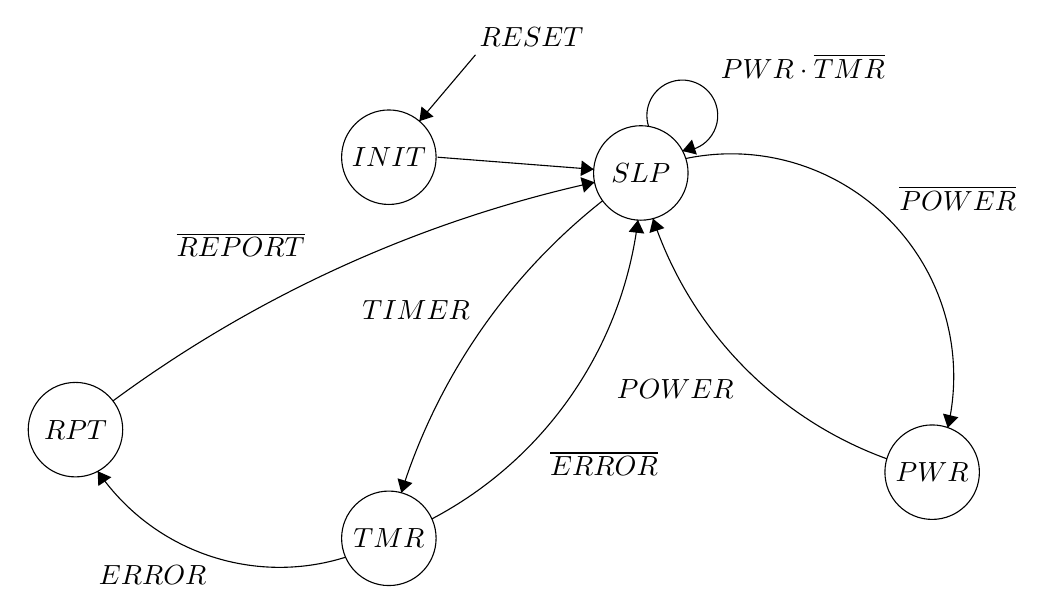
\begin{tikzpicture}[scale=0.2]
\tikzstyle{every node}+=[inner sep=0pt]
\draw [black] (31.1,-9.2) circle (3);
\draw (31.1,-9.2) node {$INIT$};
\draw [black] (47.1,-10.2) circle (3);
\draw (47.1,-10.2) node {$SLP$};
\draw [black] (31.1,-33.4) circle (3);
\draw (31.1,-33.4) node {$TMR$};
\draw [black] (11.2,-26.5) circle (3);
\draw (11.2,-26.5) node {$RPT$};
\draw [black] (65.6,-29.2) circle (3);
\draw (65.6,-29.2) node {$PWR$};
\draw [black] (34.2,-9.2) -- (44.11,-9.97);
\fill [black] (44.11,-9.97) -- (43.35,-9.41) -- (43.27,-10.4);
\draw [black] (47.597,-7.253) arc (198.16235:-89.83765:2.25);
\draw (57.39,-4.23) node [above] {$PWR \cdot \overline{TMR}$};
\fill [black] (49.74,-8.8) -- (50.66,-9.03) -- (50.35,-8.08);
\draw [black] (28.356,-34.599) arc (-72.54379:-145.70252:13.981);
\fill [black] (12.61,-29.14) -- (12.65,-30.08) -- (13.48,-29.52);
\draw (16.1,-35.09) node [below] {$ERROR$};
\draw [black] (13.581,-24.675) arc (126.41359:102.42622:80.804);
\fill [black] (44.16,-10.79) -- (43.27,-10.47) -- (43.49,-11.45);
\draw (21.69,-15.57) node [above] {$\overline{REPORT}$};
\draw [black] (36.6,-2.7) -- (33.04,-6.91);
\draw (40.16,-2.21) node [above] {$RESET$};
\fill [black] (33.04,-6.91) -- (33.94,-6.62) -- (33.17,-5.98);
\draw [black] (46.919,-13.193) arc (-6.93171:-62.25286:24.825);
\fill [black] (46.92,-13.19) -- (46.33,-13.93) -- (47.32,-14.05);
\draw (41.31,-28.65) node [right] {$\overline{ERROR}$};
\draw [black] (49.95,-9.283) arc (101.76021:-13.28801:14.139);
\fill [black] (66.59,-26.38) -- (67.26,-25.71) -- (66.29,-25.48);
\draw (63.49,-11.79) node [right] {$\overline{POWER}$};
\draw [black] (62.725,-28.351) arc (-109.96652:-161.56127:24.461);
\fill [black] (47.87,-13.1) -- (47.65,-14.01) -- (48.6,-13.7);
\draw (53.03,-23.9) node [left] {$POWER$};
\draw [black] (31.887,-30.506) arc (162.53362:128.28181:38.244);
\fill [black] (31.89,-30.51) -- (32.6,-29.89) -- (31.65,-29.59);
\draw (36.28,-18.92) node [left] {$TIMER$};
\end{tikzpicture}
\caption{Functional State Diagram: Main Unit}
\label{fig:fsd-main}
\end{figure}
\begin{table}[h!]
  \begin{tabular}{c|c}
    STATE&OUTPUTS\\
    \hline
    &\\
    INIT&$\overline{REPORT}\hbox{  }\hbox{  }\hbox{  }\overline{TIMER}\hbox{  }\hbox{  }\hbox{  }POWER\hbox{ }\hbox{  }\hbox{  }\overline{ERROR}$\\
    SLP&$\overline{REPORT}\hbox{  }\hbox{  }\hbox{  }\overline{TIMER}\hbox{  }\hbox{  }\hbox{  }POWER\hbox{ }\hbox{  }\hbox{  }\overline{ERROR}$\\
    TMR&$\overline{REPORT}\hbox{  }\hbox{  }\hbox{  }TIMER\hbox{  }\hbox{  }\hbox{  }POWER\hbox{ }\hbox{  }\hbox{  }\overline{ERROR}$\\
    RPT&$REPORT\hbox{  }\hbox{  }\hbox{  }TIMER\hbox{  }\hbox{  }\hbox{  }POWER\hbox{ }\hbox{  }\hbox{  }ERROR$\\
    PWR&$\overline{REPORT}\hbox{  }\hbox{  }\hbox{  }\overline{TIMER}\hbox{  }\hbox{  }\hbox{  }\overline{POWER}\hbox{ }\hbox{  }\hbox{  }ERROR$\\
  \end{tabular}
  \caption{Functional State Diagram Main Unit: State and Outputs}
  \label{fig:fsd-main-state-outputs}
\end{table}
\begin{table}[h!]
  \begin{tabular}{|c|}
    \hline
    Output List\\
    \hline
    REPORT = Send errors or warning via Bluetooth module\\
    TIMER = RTC ISR has been called\\
    POWER = Availability of mains power\\
    ERROR = Temperature related error has occurred\\
    \hline
  \end{tabular}
  \caption{Functional State Diagram Main Unit: Output List}
  \label{fig:fsd-main-output-list}
\end{table}
\end{center}
